\documentclass[10pt,letterpaper]{article}

\usepackage[utf8]{inputenc}
\usepackage[T1]{fontenc}
\usepackage{lmodern}
\usepackage[margin=0.45in,top=0.40in,bottom=0.40in]{geometry}
\usepackage{amsmath,amssymb,bm}
\usepackage{graphicx}
\usepackage{booktabs}
\usepackage{tabularx}
\usepackage{xcolor}
\usepackage{hyperref}
\usepackage[expansion=false]{microtype}
\usepackage{tcolorbox}
\usepackage{titlesec}
\usepackage{enumitem}

\graphicspath{{../figures/}{../../docs/engineering_reports/figures/}}

\definecolor{mdanavy}{RGB}{10, 30, 70}
\definecolor{mdablue}{RGB}{0, 110, 190}
\definecolor{darkgray}{RGB}{35, 42, 54}
\definecolor{lightbg}{RGB}{246, 250, 254}
\definecolor{bordergray}{RGB}{210, 225, 240}

\hypersetup{
    colorlinks=true,
    linkcolor=mdanavy,
    urlcolor=mdablue,
    citecolor=mdanavy
}

\pagestyle{empty}

\titleformat{\section}{\large\bfseries\color{mdanavy}}{}{0em}{}[\vspace{-0.4em}\rule{\linewidth}{0.8pt}\vspace{-0.3em}]

\tcbset{
    sharp corners,
    boxrule=0.8pt,
    colframe=mdanavy,
    colback=lightbg,
    left=6pt,right=6pt,top=5pt,bottom=5pt
}

\begin{document}

% HEADER BOX
\begin{tcolorbox}[colframe=mdanavy,colback=mdanavy,coltext=white,boxrule=0pt,top=6pt,bottom=6pt]
\begin{minipage}[c]{0.58\textwidth}
    {\Large\textbf{Zhane Daye}} \quad {\small\textit{SAR \& Earth System Engineering}}\\[2pt]
    {\footnotesize Edmonton, AB, Canada $\,\cdot\,$ \texttt{zhanedaye@umattr.ca} $\,\cdot\,$ \href{https://www.linkedin.com/in/zhane-umattr}{linkedin.com/in/zhane-umattr}}
\end{minipage}
\hfill
\begin{minipage}[c]{0.40\textwidth}
    \raggedleft
    {\large\textbf{TARGET: MDA SPACE}}\\[1pt]
    {\footnotesize\textbf{Role:} SAR Payload Systems Engineer / EO Applications Lead}\\[1pt]
    {\scriptsize MDA CHORUS™ Constellation \& Radar Mission Planning}
\end{minipage}
\end{tcolorbox}

\vspace{-4pt}

% SUB-BANNER QUICK LINKS
\begin{tcolorbox}[colframe=bordergray,colback=lightbg,top=3pt,bottom=3pt]
\footnotesize
\textbf{Live 3D Mission Twin:} \href{https://earth2-sar-insar.vercel.app}{\texttt{earth2-sar-insar.vercel.app}} $\,\vert\,$ 
\textbf{Report (PDF):} \href{https://earth2-sar-insar.vercel.app/reports/EARTH2_X_BAND_SAR_INSAR_ENGINEERING_REPORT.pdf}{\texttt{SAR\_ENGINEERING\_REPORT.pdf}} $\,\vert\,$ 
\textbf{GitHub v1.0.0:} \href{https://github.com/zrt219/earth2studio/releases/tag/v1.0.0-mission-twin}{\texttt{v1.0.0-mission-twin}}
\end{tcolorbox}

\vspace{-4pt}

% TWO-COLUMN CORE CONTENT
\noindent
\begin{minipage}[t]{0.51\textwidth}
    \section*{The Operational Bottleneck}
    \footnotesize
    As Canada's prime space contractor, MDA Space is developing **MDA CHORUS™**, a commercial Earth observation constellation combining a C-band trailing satellite with an X-band radar satellite. Operationalizing this multi-frequency system presents key challenges:
    \begin{enumerate}[leftmargin=12pt,topsep=1pt,itemsep=1pt,parsep=0pt]
        \item \textbf{Cross-Band Atmospheric Sensitivity Mismatch:} While C-band ($\lambda = 5.55\text{ cm}$) is relatively robust, X-band ($\lambda = 3.11\text{ cm}$) experiences nearly double the phase delay per millimeter of tropospheric water vapor, requiring automated differential phase screening.
        \item \textbf{Autonomous Multi-Sensor Constellation Tasking:} Bridging rapid weather-driven maritime and disaster alerts directly into satellite look-geometry and STAC order catalogs.
    \end{enumerate}

    \section*{The Engineering Solution}
    \footnotesize
    Based in Edmonton, AB, I engineered the \textbf{Earth-2 X-Band SAR \& InSAR Mission Twin}, creating an end-to-end mission planning and atmospheric correction pipeline directly applicable to CHORUS:
    \begin{itemize}[leftmargin=12pt,topsep=1pt,itemsep=1pt,parsep=0pt]
        \item \textbf{Coupled NWP-to-Radar STAC Engine:} Real-time severe weather trajectories autonomously generate OGC STAC v1.0.0 tasking orders with complete \texttt{sar:*} and \texttt{sat:*} metadata (Spotlight \& StripMap, VV/VH), sealed with SHA-256 cryptographic provenance.
        \item \textbf{Dual-Component Mesoscale APS Correction:} Evaluates Saastamoinen ZHD and Askne-Nordius ZWD across $8\times$ upsampled grids ($0.03125^\circ$), eliminating \textbf{12.20 false fringes} with a verified \textbf{98.73\% phase RMSE reduction}.
        \item \textbf{Multi-Sensor WebGL Digital Twin:} Built a 60~FPS Three.js mission twin streaming 16K global / 131K regional LOD tiles with a lightweight \textbf{248 MB GPU VRAM footprint}.
    \end{itemize}

    \section*{Verified Benchmark Record}
    \footnotesize
    \begin{tabularx}{\linewidth}{X r r}
        \toprule
        \textbf{Capability / Parameter} & \textbf{Conventional Tool} & \textbf{Engineered Twin} \\
        \midrule
        InSAR APS Phase Reduction & None / Empirical & \textbf{98.73\% to 98.81\% RMSE} \\
        False Atmospheric Fringes & 9 to 15 Fringes & \textbf{Cleanly Removed ($0.00$)} \\
        Tasking Order Format & Proprietary XML & \textbf{OGC STAC v1.0.0 GeoJSON} \\
        Atmospheric Input Grid & $0.25^\circ$ ($28\text{ km}$) & \textbf{$0.03125^\circ$ ($3.4\text{ km}$) $8\times$} \\
        Software Verification & Manual QC & \textbf{321 Pytest / 105 E2E} \\
        Deployment Platform & Desktop-only GIS & \textbf{Universal 3D WebGL (Vercel)} \\
        \bottomrule
    \end{tabularx}
\end{minipage}
\hfill
\begin{minipage}[t]{0.46\textwidth}
    \section*{Visual Mission Twin Artifact}
    \centering
    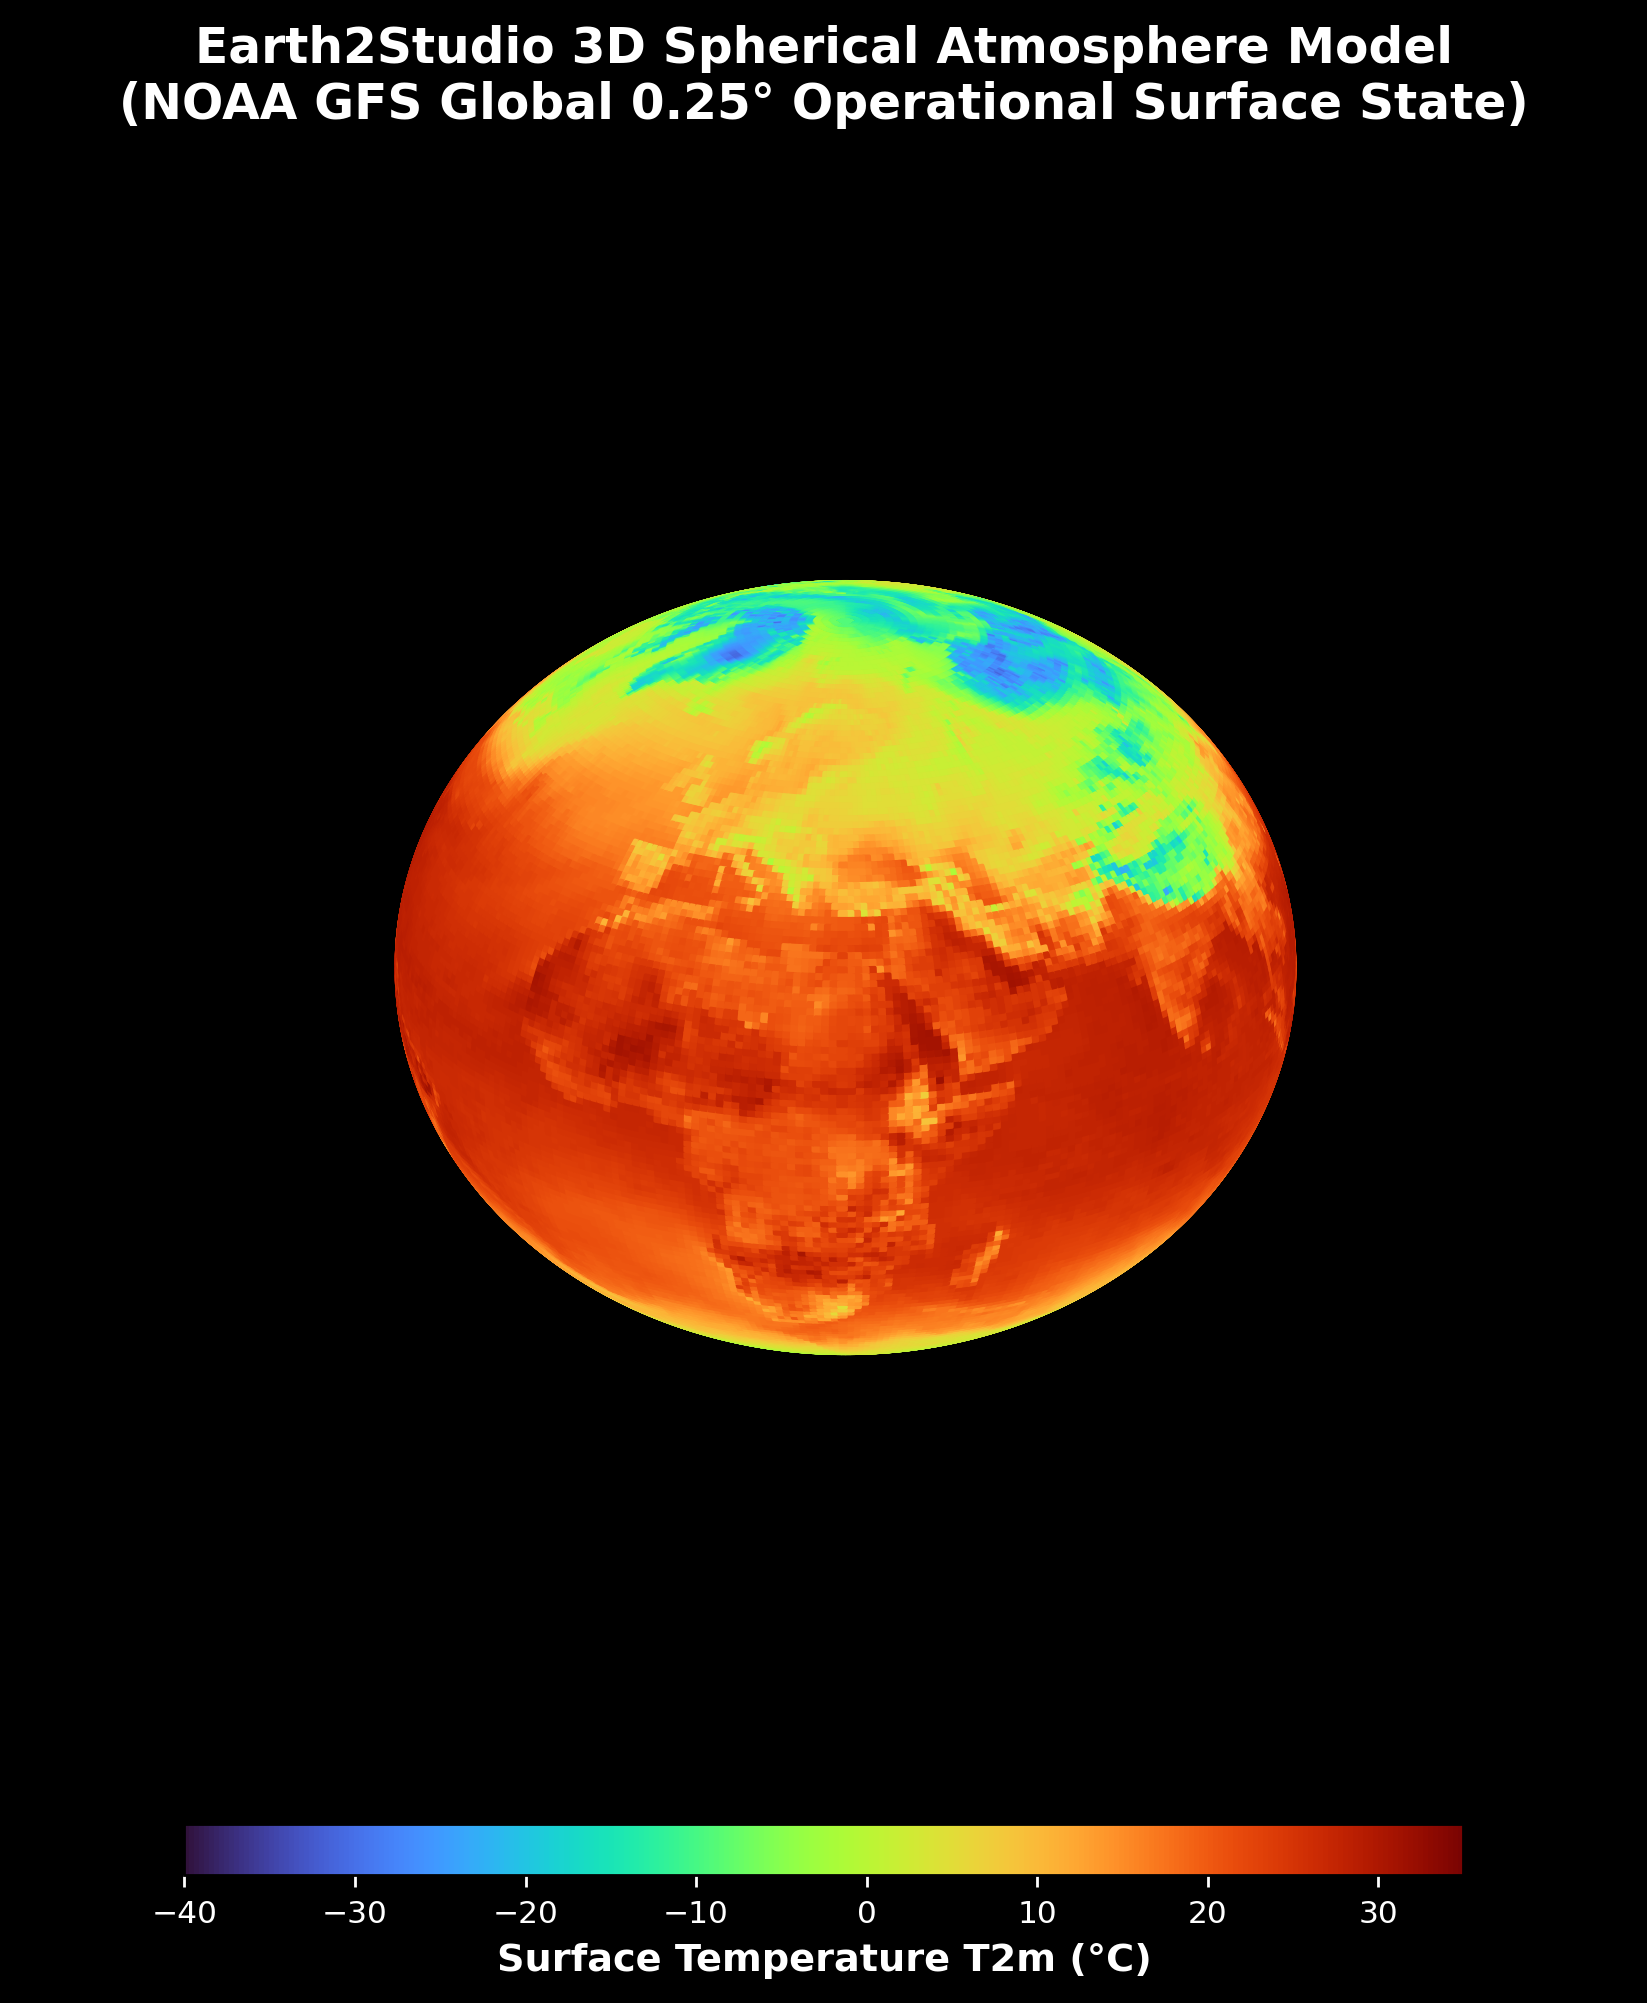
\includegraphics[width=\linewidth,height=1.75in,keepaspectratio]{earth_3d_spherical_model.png}\\[2pt]
    {\scriptsize\textit{Figure: 3D Spherical Mission Twin ($R=5.000\rightarrow 5.420$) rendering dynamic satellite orbit arcs, slant-range look-frustums, and real-time atmospheric fields.}}

    \vspace{2pt}

    \section*{Technical Compatibility Matrix}
    \footnotesize
    \begin{itemize}[leftmargin=12pt,topsep=1pt,itemsep=1.5pt,parsep=0pt]
        \item \textbf{Radar Systems Engineering:} SAR payload link budget, Doppler centroid, slant-range to ground-range conversion, multi-polarization (VV/VH/HH), SAR interferometry.
        \item \textbf{Spaceflight Operations:} Sun-Synchronous Orbits (SSO), Keplerian orbit propagation, ground-station coverage, OGC STAC v1.0.0 tasking.
        \item \textbf{Atmospheric Modeling:} NVIDIA Earth2Studio, NOAA GFS, Saastamoinen hydrostatic delay, wet refractivity integration.
        \item \textbf{Software Quality:} Python 3.10+, Pytest (321 passed), WebGL 2.0, Three.js, GitHub CI/CD, Canadian Controlled Goods eligibility.
    \end{itemize}

    \section*{Direct Value to MDA Space}
    \footnotesize
    \begin{tcolorbox}[colframe=mdablue,colback=white,boxrule=0.6pt,top=4pt,bottom=4pt]
    \textbf{Immediate Operational Impact:}
    \begin{itemize}[leftmargin=10pt,topsep=0pt,itemsep=1pt]
        \item Canadian citizen / resident in Edmonton, AB, available for engineering roles supporting Richmond, BC or Brampton, ON programs.
        \item Ready-to-integrate algorithms for CHORUS multi-frequency cross-calibration and automated tasking.
        \item Strong software engineering foundation with verified test automation and publication-grade technical documentation.
    \end{itemize}
    \end{tcolorbox}
\end{minipage}

\vspace{-2pt}

% FOOTER CALL TO ACTION
\begin{tcolorbox}[colframe=mdanavy,colback=mdanavy,coltext=white,boxrule=0pt,top=4pt,bottom=4pt]
\centering\footnotesize
\textbf{Explore the Interactive Demo:} \href{https://earth2-sar-insar.vercel.app}{\texttt{earth2-sar-insar.vercel.app}} $\,\cdot\,$ 
\textbf{Contact Zhane Daye:} \texttt{zhanedaye@umattr.ca} $\,\cdot\,$ Available for technical review \& interviews.
\end{tcolorbox}

\end{document}
